\documentclass[tikz,border=10pt]{standalone}
\usetikzlibrary{shapes.geometric, arrows.meta, bending}

\definecolor{basepurple}{RGB}{102,43,240}
\definecolor{basered}{RGB}{218,58,50}
\definecolor{basegreen}{RGB}{92,214,41}
\definecolor{baseteal}{RGB}{41,230,229}


\begin{document}
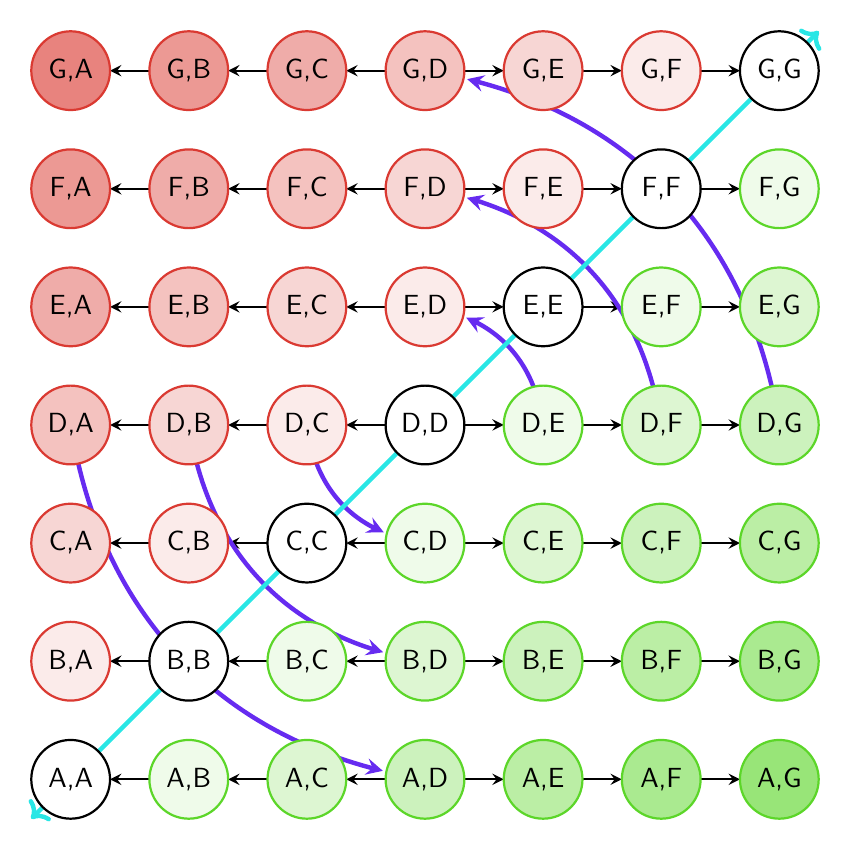
\begin{tikzpicture}[font=\sffamily]
  \tikzset{
    green_circle/.style args={#1}{
      circle, draw=basegreen, fill=basegreen!#1!white, thick, minimum size=1cm, inner sep=0pt
    },
    red_circle/.style args={#1}{
      circle, draw=basered, fill=basered!#1!white, thick, minimum size=1cm, inner sep=0pt
    },
    empty_circle/.style args={#1}{
      circle, draw=black, fill=white, thick, minimum size=1cm, inner sep=0pt
    },
    arrow_arc/.style={->, >=stealth, ultra thick, shorten >=12pt},
    connecting_arrow/.style={->, >=stealth, thick}
  }
  
\foreach \y [count=\yi] in {A,...,G} {
  \foreach \x [count=\xi] in {A,...,G} {
    \node[] (H-\x-\y) at (1.5*\xi-6,1.5*\yi-6) {};

  \ifnum\xi>4
    \draw[connecting_arrow] (1.5*\xi-7.0,1.5*\yi-6) -- (1.5*\xi-6.5,1.5*\yi-6);
  \else
    \ifnum\xi>1
      \draw[connecting_arrow] (1.5*\xi-6.5,1.5*\yi-6) -- (1.5*\xi-7.0,1.5*\yi-6);
    \fi
  \fi
  }    
}

\foreach \x [count=\xi] in {A,...,G} {
  \ifnum\xi=4
  \else
    \draw[arrow_arc, basepurple, bend right=35] (H-\x-D) to (H-D-\x);
  \fi
}

\draw[baseteal, ultra thick, <->] (-5, -5) -- (5, 5);

  % Draw the grid of nodes and adjust tint based on distance from the teal line
  \foreach \y [count=\yi] in {A,...,G} {
    \foreach \x [count=\xi] in {A,...,G} {
      % Calculate dot product with the orthogonal vector (1, -1)
      \pgfmathsetmacro{\dotproduct}{(1.5*\xi-6) - (1.5*\yi-6)};
      \pgfmathtruncatemacro{\tintcheck}{\dotproduct * 7};
      \pgfmathtruncatemacro{\tint}{abs(\dotproduct) * 7};
      
      \ifnum\tintcheck>0
        \node[green_circle=\tint] (H-\x-\y) at (1.5*\xi-6,1.5*\yi-6) {\y,\x};
      \else
        \ifnum\tintcheck<0
            \node[red_circle=\tint] (H-\x-\y) at (1.5*\xi-6,1.5*\yi-6) {\y,\x};
        \else
            \node[empty_circle=\tint] (H-\x-\y) at (1.5*\xi-6,1.5*\yi-6) {\x,\x};
        \fi
      \fi
    }
  }

\end{tikzpicture}
\end{document}